% ITU journal article template

\documentclass[a4paper,twocolumn]{article}

\usepackage{fontspec}
\usepackage{unicode-math}
\usepackage{authblk}
\usepackage{graphicx}
\usepackage[explicit]{titlesec}
\usepackage[labelfont=bf,labelsep=endash,font=footnotesize]{caption}
\usepackage{tabu}
\usepackage{xcolor}
\usepackage[backend=biber,natbib=true,style=numeric,maxnames=50,sorting=none]{biblatex}
\usepackage[hidelinks]{hyperref}
\usepackage[hang]{footmisc}
\usepackage{abstract}
\usepackage{mathtools}
\usepackage{parskip}
\usepackage{balance}
\usepackage{wrapfig}
\usepackage{lineno}

\hypersetup{
	colorlinks = true,
	urlcolor= blue,
	linkcolor = blue,
	citecolor=.
}

% add bibliography file
\addbibresource{ituJournalPaper.bib}

\title{Template for submitting papers to the ITU journal on Future and Evolving Technologies (ITU J-FET)}

% Please spell out first names and surnames
\author[1]{\normalsize{Author's name}}
\author[2]{\normalsize{second author's name}}

\affil[1]{\normalsize{First author's affiliation and full address}}
\affil[2]{\normalsize{Second author's affiliation and full address, etc.}}

\begin{document}

\twocolumn[
\begin{@twocolumnfalse}
\maketitle

\begin{abstract}
This template provides detailed instructions for submitting papers to ITU J-FET.
Papers must be in English and in black font, no page limit.
The abstract should appear in italics at the top, below the title and author's area. 
The abstract should normally contain 150 to 200 words, and in no case shall it exceed 300 words.
All abbreviations and acronyms used in the abstract should be defined, and in the text the first time used.
Do not cite references in the abstract.
\end{abstract}
\end{@twocolumnfalse}
]

% the below command can be used to change the start of page numbering
\setcounter{page}{1}

\section{Introduction} 
\label{sec:intro}
This template provides detailed instructions for submitting papers to ITU J-FET. The next sections describe style, fonts and spacing to adopt. Please use this \LaTeX\ template for your paper. 

Additional instructions on submitting your paper can be found in the \href{https://www.itu.int/en/journal/Pages/submission-guidelines.aspx}{Author's Guidelines}. Please address any enquiries or suggestions about this template to the ITU Journal Team at \href{mailto:journal@itu.int}{journal@itu.int}.


\section{Formatting}
\label{sec:sec2}
All text, illustrations and charts must be kept within a print area of 17.5 cm/6.9 inches wide by 24.4 cm/9.6 inches high.
Do not write anything outside the print area.
The top margin must be 2.5 cm, and the left and right margins must be 1.5 cm.
All text must be in a two-column format.
Columns are to be 8.5 cm wide, with a 1 cm space between them.
Text must be fully justified, A4 size (21 cm wide by 29.7 cm long, or 8.27 inches by 11.7 inches).

If the last page of your paper is only partially filled, arrange the columns so that they are evenly balanced if possible, rather than having one long column.
The balancing can be achieved using the \texttt{\textbackslash balance} command before the last section of the left column of the last page.


\section{Title page section}
\label{sec:sec3}
The paper title should be \texttt{Large} size, uppercase, and bold face, as shown in this template.
The authors' name(s) and affiliation(s) are to appear below the title in capital and lower case letters, in \texttt{large} size, keeping the spacing as indicated in the template instructions.


\section{Type-style and fonts}
\label{sec:sec4}
Text should appear in Cambria font, size 10-point, with single spacing, apart from headings.
This is already implemented as default in the template.
To be able to obtain the Cambria character \textbf{compile using XeLaTeX}, instead of pdflatex.


\section{Major headings}
\label{sec:sec5}
Major headings (for example, ``1. INTRODUCTION'') are predefined in the template, and \textbf{should not} be changed.

\subsection{Subheadings}
\label{ssec:sec5.1}
Subheadings are predefined in the template, and \textbf{should not} be changed.

\subsubsection{Sub-subheading}
\label{sssec:sec5.1.1}
Sub-subheadings, as in this paragraph, are discouraged.
However, if you must use them, they should appear as predefined in the template, and \textbf{should not} be changed.


\section{Images}
\label{sec:sec6}
Images (figures and tables) can be either in color or black and white.
Images must appear within the designated margins.
Caption and number every image.
Figure captions must be placed on the bottom, not top, of the figure.
Table captions must be located on the top of the table.
Keep titles with images. 

\begin{figure}
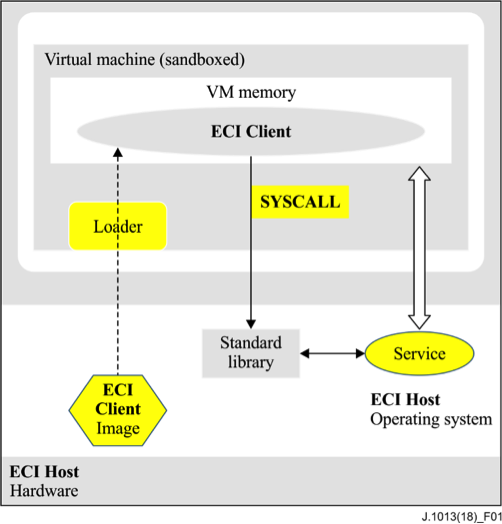
\includegraphics[width=\columnwidth]{Figure1}
\caption{ECI Host - Hardware}\label{fig:fig1} 
\end{figure}

And for a table:

\begin{table}
\caption{Table title style}\label{tab:tab1} 
\begin{small}
\begin{tabu}{|c|c|}
\hline
 \rowfont{\bfseries}Character & Entity Reference\\ 
  & \\
\hline
\hline
\& & \&amp; \\
\hline
 < & \&lt;\\
 \hline
 > & \&gt; \\
\hline
``  & \&quot; \\
\hline
 ` & \&apos; \\
\hline
\end{tabu}
\end{small}
\end{table}

And an equation:
\begin{equation}\label{eq:eq1}
PL(D)=PL(D)+10\log 
\end{equation}

%\balance

\section{Footnotes}
\label{sec:sec7}
Use footnotes sparingly (or not at all!)\footnote{To obtain the right formatting for the footnotes}.
To help your readers, avoid using footnotes altogether and include necessary peripheral observations in the text (within parentheses, if you prefer, as in this sentence).


\section{Using references}
\label{sec:sec8}
List and number all bibliographical references at the end of the paper, and refer to them in the text as shown in this sentence \cite{author2021}.


\section{Page numbering}
\label{sec:sec9}
Please number all pages of your paper.


\section{Authoring recommendations}
\label{sec:sec10}
Define abbreviations and acronyms the first time they are used in the text, even if they have already been defined in the abstract.
Abbreviations and acronyms should be avoided in the title.
Units should be expressed as much as possible in international units, and a dot (``.'') should be used to express decimal points (not ``,'').


\section{Conclusion}
\label{sec:sec11}
The main conclusions may be presented in a short final section.


\section*{Acknowledgements}
\label{sec:ackn}
You may list here colleagues, sponsors and financial supporter that you wish to acknowledge.
This section is not required.


\printbibliography 


\section*{Authors}
\label{sec:auth}


\includegraphics[]{yourphotofilename.jpg} 
\textbf{First A. Author} Biographies should be limited to one paragraph consisting of the following: sequentially ordered list of degrees, including years achieved; sequentially ordered places of employ concluding with current employment; association with any official journals or conferences; major professional and/or academic achievements, i.e., best paper awards, research grants, etc.; any publication information (number of papers and titles of books published); current research interests; association with any professional associations.


\includegraphics{yourphotofilename.jpg}
\textbf{Second A. Author} Biographies should be limited to one paragraph consisting of the following: sequentially ordered list of degrees, including years achieved; sequentially ordered places of employ concluding with current employment; association with any official journals or conferences; major professional and/or academic achievements, i.e., best paper awards, research grants, etc.; any publication information (number of papers and titles of books published); current research interests; association with any professional associations.


\includegraphics[width=0.39\columnwidth]{yourphotofilename.jpg} 
\textbf{Third A. Author} Biographies should be limited to one paragraph consisting of the following: sequentially ordered list of degrees, including years achieved; sequentially ordered places of employ concluding with current employment; association with any official journals or conferences; major professional and/or academic achievements, i.e., best paper awards, research grants, etc.; any publication information (number of papers and titles of books published); current research interests; association with any professional associations.

\end{document}